\documentclass[a4paper, twocolumn]{article}
\usepackage[pdftex, hidelinks]{hyperref}

\usepackage{bm}
\usepackage[T1]{fontenc}
\usepackage[utf8]{inputenc}
\usepackage{algpseudocode}
\usepackage{algorithm}
\usepackage{amsfonts}
\usepackage{amssymb}
\usepackage{courier}
\usepackage{booktabs}
\usepackage{graphicx}
\usepackage{listings}
\usepackage{mathtools}
\lstset{basicstyle=\footnotesize\ttfamily,
        breakatwhitespace = false,
        breaklines = true,
        keepspaces = true,
        language = R,
        showspaces = false,
        showstringspaces = false,
        belowcaptionskip = \bigskipamount,
        framerule = 0.80pt,
        frame = tb,
        belowskip = \bigskipamount,
        escapeinside={<@}{@>}}

\title{TDDE01 -- Machine Learning \\
       Group 9 Laboration Report 1}
\author{{Martin Estgren \texttt{<mares480>}} \\
        {Björn Jansson \texttt{<bjoja408>}} \\
        {Erik S. V. Jansson \texttt{<erija578>}} \\
        {Sebastian Maghsoudi \texttt{<sebma654>}} \\~\\
        {Linköping University (LiU), Sweden}}

\begin{document}
    \pagenumbering{arabic}
    \maketitle % Generate.

    \section*{Assignment 1}

    Nobody likes \emph{e-mail spam}, therefore methods for autonomously \emph{predicting} if a given e-mail is probably \emph{spam} or \emph{not spam} is an important task. This is a classic example where \emph{machine learning} is useful; given a set of \emph{training data} and \emph{testing data}, can we predict what is \emph{spam} and \emph{not spam} in the \emph{testing set} (without knowing the answer) by deriving a \emph{hypothesis function} built from the \emph{training data}?

    By using \emph{k-nearest neighbor classification}, one can derive if an e-mail is spam or not by simply looking at \emph{similar e-mails/messages}, and picking the most likely solution by doing a \emph{``majority vote''}. First, a \emph{distance function} needs to be implemented, which is the \emph{cosine distance function} in Equation~\ref{eq:distance}, whose implementation can be found in Listing~\ref{lst:distance}, but with a optimized solution using only matrices.

    \begin{equation} \label{eq:distance}
        d(X,Y) = 1 - \frac{X^TY}{\sqrt{\sum_i{X_i^2}}\sqrt{\sum_i{Y_i^2}}}
    \end{equation}

    After defining the distance function $d(X,Y)$, one can find the \emph{e-mail/message distance} for each $Y_j$ in respect to each $X_i$. Where $X$ is the \emph{testing set} and $Y$ the \emph{training set}. Each row of the resulting matrix contains the relative distance between $X_i$ and $\forall Y_j$. Therefore, sorting each row $X_i$ and picking the first $K$ elements gives the $K$ \emph{closest messages} from the \emph{training set} in respect to each \emph{testing element}. By using this, the \emph{k-nearest neighbors} can be found, and the prediction of $\hat{Y}$ (spam, not spam) is done by using Equation~\ref{eq:knn}, where $K_i$ classify as being $C_i$.

    \begin{equation} \label{eq:knn}
        \hat{Y} = \underset{\forall C_i}{\mathrm{max}}\; p(C_i | \bm{x}),\; p(C_i | \bm{x}) \propto K_i \div K
    \end{equation}

    The \emph{k-nearest neighbor algorithm} is implemented in Listing~\ref{lst:knearest}, in the function \texttt{knearest(t,k,t')}. It works as previously described, where line \texttt{20} is calculating the \emph{distance matrix} and line \texttt{21} sorting each row, so that all $Y$ distances are relative to $X_i$. Thereafter, in line \texttt{26-27} the classification is found for the $K$-nearest neighbors of $X_i$. The \emph{mean} value is then taken, which is equivalent to $K_i \div K$ since only two classifications exist (spam and not spam), following a \emph{Cover et al.}~\cite{cover1967nearest} K-NN descriptions.

    From the \textit{knearest} function we get a vector containing all the predicted classifications for the data set. First we set a probability threshold \( p(\mathbf{x} |\theta) > 0.5\) and compare the predicted classifications with the true classifications in the data set. Where the threshholds are done in lines \texttt{49-50} in the main spam classification script found under a Listing~\ref{lst:spam}.

    The result for \(k = 5,\, k = 1\) can be observed in the following tables, for both \emph{kknn} and \emph{knearest.r}:
\begin{verbatim}
            knearest, k = 5
observations   0   1
           0 682 263
           1 186 239
misclassification rate = 0.3277372
\end{verbatim}
    These results indicate a ``hit ratio'' of around \(68 \%\).

\begin{verbatim}
            knearest, k = 1
observations   0   1
           0 650 295
           1 174 251
misclassification rate = 0.3423358
\end{verbatim}
    These results indicate a ``hit ratio'' of around \(66 \%\) for the results when \emph{knearest} has $k=1$ neighbors.

    The result indicates that our classifier is fairly good for the given data set but to get a better perspective we compare it to a built in classifier called \textit{Weighted K-nearest neighbor} (kknn) on the same training and testing data set. The result can be observed bellow,\, for both $k=1$ and $k=5$ values:

\begin{verbatim}
            kknn, k = 5, k = 1
observations   0   1
           0 626 319
           1 184 241
misclassification rate = 0.3671533
\end{verbatim}
    The biggest difference from out own implementation is that the hit rate and confusion matrix are identical for both \(K = 1\) and \(K = 5\). The hit rate is also slightly lower that ours at about \( 0.63\).

    We then proceed to plot the classifiers in a \textit{ROC - curve} for the probability threshold \( p(x) > 0.05,...,0.95\) with steps of \(0.01\). Where the \emph{x-axis} shows the \emph{sensitivity}/\emph{true positive rate} and the \emph{y-axis} shows the \emph{false negative rate}. 
The \textit{true positive rate} is calculated as
\begin{equation}
 \frac{Tp}{Tp + Fn}
\end{equation}
where \(Tp\) stands for the \textit{true positives} i.e. the cases where both the prediction and observations classified the case as \textit{true}, and \(Fn\) stands for the \textit{false negatives} i.e. the cases where the prediction was \textit{false} but the observation was \textit{true}.

The \textit{true negative rate} is calculated as \(1 - specificity\) where \textit{specificity} is equal to:
\begin{equation}
 \frac{Tn}{Tn + Fp}
\end{equation}
where \(Tn\) stands for the \textit{true negatives} i.e. the cases where both the prediction and observations classified the case as \textit{false}, and \(Fp\) stands for the \textit{false positives} i.e. the cases where the prediction was \textit{true} but the observation was \textit{false}.

These operations can be found in the lines \texttt{95-97} for \emph{knearest} and \texttt{109-111} for \emph{kknn} in Listing~\ref{lst:spam} \texttt{spam.r}.

    The resulting \textit{ROC - curve} can be observed in the column to the right, that is in the Figure~\ref{fig:roc}.

    Blue curve is \textit{knearest} and green curve is \textit{kknn}. The red line is a reference line for a random classifier. The result indicates as with the confusion matrices that our \textit{knearest} implementation slightly out performs \textit{kknn} on some threshold variables.

\begin{figure}[H]
\centering
\begin{minipage}[]{0.5\textwidth}
  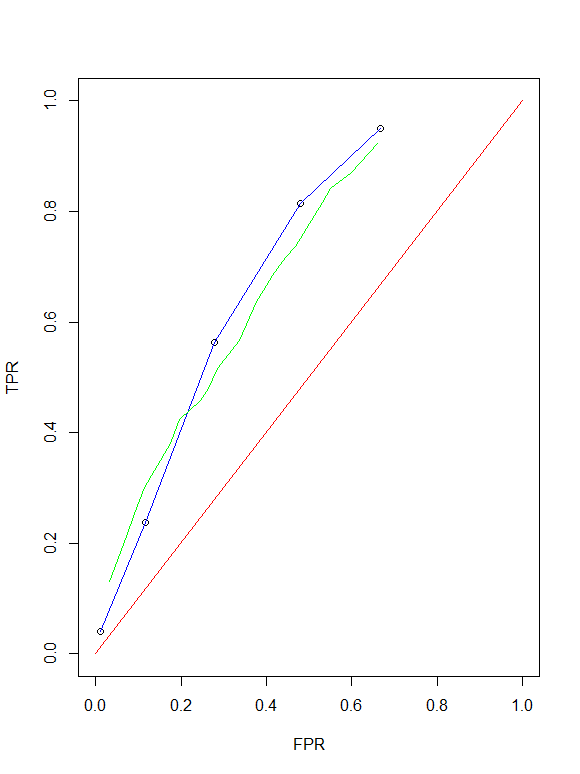
\includegraphics[width=\textwidth]{share/Lab1_A1_ROC.png}  
  \caption{ROC - curve of  \textit{knearest} and  \textit{kknn}.\label{fig:roc} }
 \end{minipage}
\end{figure}

    \section*{Assignment 2}

    ...

    \section*{Contributions}

    \begin{itemize}
        \item{\textbf{Erik S. V. Jansson:} wrote the initial section in \emph{Assignment 1} regarding on how the \emph{k-nearest neighbor algorithm} works, and also provided the \texttt{knearest} scripts in Listings~\ref{lst:knearest},\ref{lst:distance}. Additionally, he also extended the formula description on \emph{ROC-curves} for full completeness.}
        \item{\textbf{Martin Estgren:} wrote the sections on generating \emph{confusion matrices} and the \emph{missclassification ratio} of \emph{knearest} and \emph{kknn}. Additionally, on how to generate \emph{ROC-curves} and the plot itself. Finally, he provided Listing~\ref{lst:spam} which wraps the script functions in assignment 1 up.}
    \end{itemize}

    \nocite{*} % No warnings.
    \bibliographystyle{alpha}
    \bibliography{report}
    \onecolumn \appendix
    \section*{Appendix}

    \lstinputlisting[caption={K-Nearest Neighbor Algorithm Implementation},label={lst:knearest}]{share/knearest.r}
    \lstinputlisting[caption={Cosine Cost/Distance Formula},label={lst:distance}]{share/distance.r}
    \lstinputlisting[caption={Main Spam Prediction Script},label={lst:spam}]{share/spam.r}

\end{document}
